% Options for packages loaded elsewhere
% Options for packages loaded elsewhere
\PassOptionsToPackage{unicode}{hyperref}
\PassOptionsToPackage{hyphens}{url}
\PassOptionsToPackage{dvipsnames,svgnames,x11names}{xcolor}
%
\documentclass[
  12pt,
  letterpaper,
  DIV=11,
  numbers=noendperiod]{scrartcl}
\usepackage{xcolor}
\usepackage[left=25mm,right=25mm,top=25mm,bottom=25mm]{geometry}
\usepackage{amsmath,amssymb}
\setcounter{secnumdepth}{-\maxdimen} % remove section numbering
\usepackage{iftex}
\ifPDFTeX
  \usepackage[T1]{fontenc}
  \usepackage[utf8]{inputenc}
  \usepackage{textcomp} % provide euro and other symbols
\else % if luatex or xetex
  \usepackage{unicode-math} % this also loads fontspec
  \defaultfontfeatures{Scale=MatchLowercase}
  \defaultfontfeatures[\rmfamily]{Ligatures=TeX,Scale=1}
\fi
\usepackage{lmodern}
\ifPDFTeX\else
  % xetex/luatex font selection
\fi
% Use upquote if available, for straight quotes in verbatim environments
\IfFileExists{upquote.sty}{\usepackage{upquote}}{}
\IfFileExists{microtype.sty}{% use microtype if available
  \usepackage[]{microtype}
  \UseMicrotypeSet[protrusion]{basicmath} % disable protrusion for tt fonts
}{}
\makeatletter
\@ifundefined{KOMAClassName}{% if non-KOMA class
  \IfFileExists{parskip.sty}{%
    \usepackage{parskip}
  }{% else
    \setlength{\parindent}{0pt}
    \setlength{\parskip}{6pt plus 2pt minus 1pt}}
}{% if KOMA class
  \KOMAoptions{parskip=half}}
\makeatother
% Make \paragraph and \subparagraph free-standing
\makeatletter
\ifx\paragraph\undefined\else
  \let\oldparagraph\paragraph
  \renewcommand{\paragraph}{
    \@ifstar
      \xxxParagraphStar
      \xxxParagraphNoStar
  }
  \newcommand{\xxxParagraphStar}[1]{\oldparagraph*{#1}\mbox{}}
  \newcommand{\xxxParagraphNoStar}[1]{\oldparagraph{#1}\mbox{}}
\fi
\ifx\subparagraph\undefined\else
  \let\oldsubparagraph\subparagraph
  \renewcommand{\subparagraph}{
    \@ifstar
      \xxxSubParagraphStar
      \xxxSubParagraphNoStar
  }
  \newcommand{\xxxSubParagraphStar}[1]{\oldsubparagraph*{#1}\mbox{}}
  \newcommand{\xxxSubParagraphNoStar}[1]{\oldsubparagraph{#1}\mbox{}}
\fi
\makeatother


\usepackage{longtable,booktabs,array}
\usepackage{calc} % for calculating minipage widths
% Correct order of tables after \paragraph or \subparagraph
\usepackage{etoolbox}
\makeatletter
\patchcmd\longtable{\par}{\if@noskipsec\mbox{}\fi\par}{}{}
\makeatother
% Allow footnotes in longtable head/foot
\IfFileExists{footnotehyper.sty}{\usepackage{footnotehyper}}{\usepackage{footnote}}
\makesavenoteenv{longtable}
\usepackage{graphicx}
\makeatletter
\newsavebox\pandoc@box
\newcommand*\pandocbounded[1]{% scales image to fit in text height/width
  \sbox\pandoc@box{#1}%
  \Gscale@div\@tempa{\textheight}{\dimexpr\ht\pandoc@box+\dp\pandoc@box\relax}%
  \Gscale@div\@tempb{\linewidth}{\wd\pandoc@box}%
  \ifdim\@tempb\p@<\@tempa\p@\let\@tempa\@tempb\fi% select the smaller of both
  \ifdim\@tempa\p@<\p@\scalebox{\@tempa}{\usebox\pandoc@box}%
  \else\usebox{\pandoc@box}%
  \fi%
}
% Set default figure placement to htbp
\def\fps@figure{htbp}
\makeatother





\setlength{\emergencystretch}{3em} % prevent overfull lines

\providecommand{\tightlist}{%
  \setlength{\itemsep}{0pt}\setlength{\parskip}{0pt}}



 


\usepackage{indentfirst}
\setlength{\parindent}{15pt}
\setlength{\parskip}{10pt}
\usepackage[font=small]{caption}
\usepackage[noblocks]{authblk}
\renewcommand*{\Authsep}{, }
\renewcommand*{\Authand}{, }
\renewcommand*{\Authands}{, }
\renewcommand\Affilfont{\small}
\KOMAoption{captions}{tablesignature}
\makeatletter
\@ifpackageloaded{caption}{}{\usepackage{caption}}
\AtBeginDocument{%
\ifdefined\contentsname
  \renewcommand*\contentsname{Table of contents}
\else
  \newcommand\contentsname{Table of contents}
\fi
\ifdefined\listfigurename
  \renewcommand*\listfigurename{List of Figures}
\else
  \newcommand\listfigurename{List of Figures}
\fi
\ifdefined\listtablename
  \renewcommand*\listtablename{List of Tables}
\else
  \newcommand\listtablename{List of Tables}
\fi
\ifdefined\figurename
  \renewcommand*\figurename{Figure}
\else
  \newcommand\figurename{Figure}
\fi
\ifdefined\tablename
  \renewcommand*\tablename{Table}
\else
  \newcommand\tablename{Table}
\fi
}
\@ifpackageloaded{float}{}{\usepackage{float}}
\floatstyle{ruled}
\@ifundefined{c@chapter}{\newfloat{codelisting}{h}{lop}}{\newfloat{codelisting}{h}{lop}[chapter]}
\floatname{codelisting}{Listing}
\newcommand*\listoflistings{\listof{codelisting}{List of Listings}}
\makeatother
\makeatletter
\makeatother
\makeatletter
\@ifpackageloaded{caption}{}{\usepackage{caption}}
\@ifpackageloaded{subcaption}{}{\usepackage{subcaption}}
\makeatother
\usepackage{bookmark}
\IfFileExists{xurl.sty}{\usepackage{xurl}}{} % add URL line breaks if available
\urlstyle{same}
\hypersetup{
  pdftitle={Adaptation to orientation in natural scenes},
  pdfauthor={Bruno Richard; Patrick Shafto},
  colorlinks=true,
  linkcolor={blue},
  filecolor={Maroon},
  citecolor={Blue},
  urlcolor={Blue},
  pdfcreator={LaTeX via pandoc}}


\title{Adaptation to orientation in natural scenes}
\author{Bruno Richard \and Patrick Shafto}
\date{}
\begin{document}
\maketitle
\begin{abstract}
The encoding mechanisms of the human visual system are associated with
the distribution of features in natural environments (Olshausen \&
Field, 2000). Moreover, exposure to modified environments over an hour
or so can generate meaningful changes in the visual sensitivity of
observers, suggesting the importance of recent experience (Richard \&
Shafto, 2022, Schweinhart, Shafto, \& Essock, 2017). This work measured
sensitivity to the features of natural environments (e.g., orientation
contrast and the slope of the amplitude spectrum) before and following
the 60-minute adaptation period, which gives little indication of the
time course of adaptation in modified environments. Here, we use the
horizontal effect; an orientation anisotropy thought to be related to
the distribution of orientation contrast in natural environments, to
monitor the time course of adaptation in modified reality. We measured
sensitivity to orientation with a matching task in nine observers.
Observers wore a Head-Mounted Display (HMD) that presented an unaltered
or an isotropic version of their environment, recorded from a
head-mounted camera. Sensitivity to orientation was measured in the HMD
with an orientation and contrast matching task. Before adaptation,
observers exhibited the expected anisotropy; sensitivity to horizontally
oriented stimuli was worse than vertical and oblique stimuli. During the
first half of the adaptation period, sensitivity to horizontal stimuli
improved, matching that of other orientations within 30 minutes of
immersion in the isotropic environment. Sensitivity to different
orientations was unaffected by the isotropic environment. Our findings
demonstrate that adaptation to a novel, isotropic environment occurs
gradually over a relatively brief time of approximately 30 minutes.
Additionally, we bring further evidence that human sensitivity to
oriented content is associated with the distribution of orientation
contrast in the current environment of observers.
\end{abstract}


\section{Introduction}\label{introduction}

The encoding mechanisms of the human visual system are associated with
the distribution of features in natural environments (Olshausen \&
Field, 2000). Moreover, exposure to modified environments over an hour
or so can generate meaningful changes in the visual sensitivity of
observers, suggesting the importance of recent experience (Richard \&
Shafto, 2022, Schweinhart, Shafto, \& Essock, 2017). This work measured
sensitivity to the features of natural environments (e.g., orientation
contrast and the slope of the amplitude spectrum) before and following
the 60-minute adaptation period, which gives little indication of the
time course of adaptation in modified environments. Here, we use the
horizontal effect; an orientation anisotropy thought to be related to
the distribution of orientation contrast in natural environments, to
monitor the time course of adaptation in modified reality. We measured
sensitivity to orientation with a matching task in nine observers.
Observers wore a Head-Mounted Display (HMD) that presented an unaltered
or an isotropic version of their environment, recorded from a
head-mounted camera. Sensitivity to orientation was measured in the HMD
with an orientation and contrast matching task. Before adaptation,
observers exhibited the expected anisotropy; sensitivity to horizontally
oriented stimuli was worse than vertical and oblique stimuli. During the
first half of the adaptation period, sensitivity to horizontal stimuli
improved, matching that of other orientations within 30 minutes of
immersion in the isotropic environment. Sensitivity to different
orientations was unaffected by the isotropic environment. Our findings
demonstrate that adaptation to a novel, isotropic environment occurs
gradually over a relatively brief time of approximately 30 minutes.
Additionally, we bring further evidence that human sensitivity to
oriented content is associated with the distribution of orientation
contrast in the current environment of observers.

\section{Methods}\label{methods}

\section{Results}\label{results}

\begin{verbatim}
[1]  0.00000 15.77778 30.88889 61.11111
\end{verbatim}

\pandocbounded{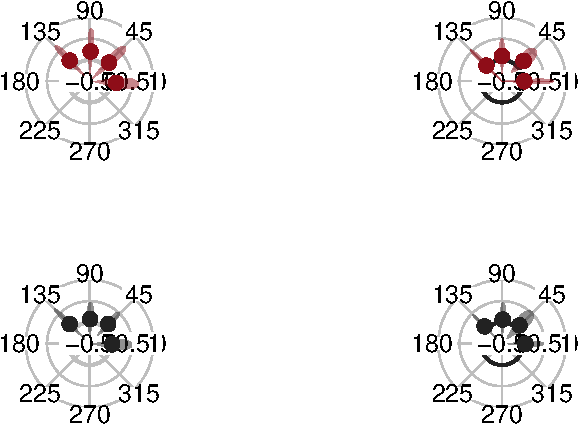
\includegraphics[keepaspectratio]{OrientationAdaptationPaper_files/figure-pdf/draw data radial-1.pdf}}

\pandocbounded{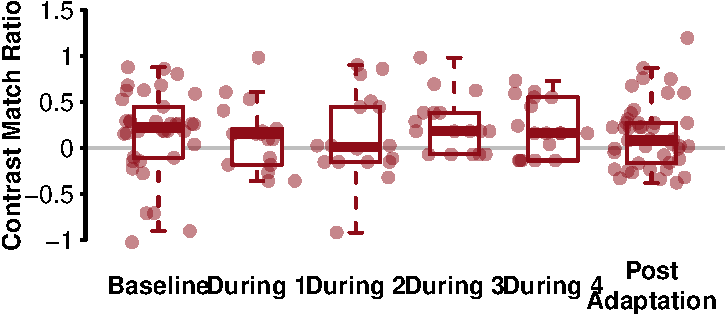
\includegraphics[keepaspectratio]{OrientationAdaptationPaper_files/figure-pdf/draw data boxplots-1.pdf}}

\pandocbounded{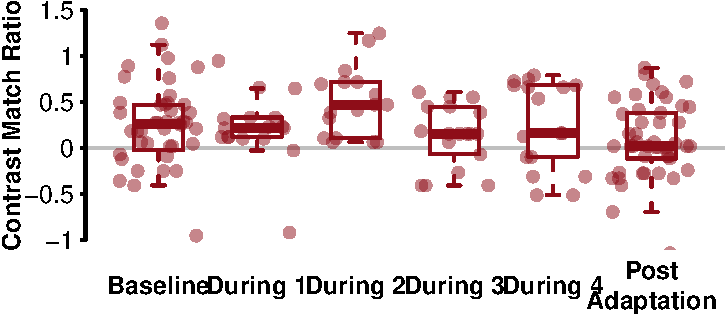
\includegraphics[keepaspectratio]{OrientationAdaptationPaper_files/figure-pdf/draw data boxplots-2.pdf}}

\pandocbounded{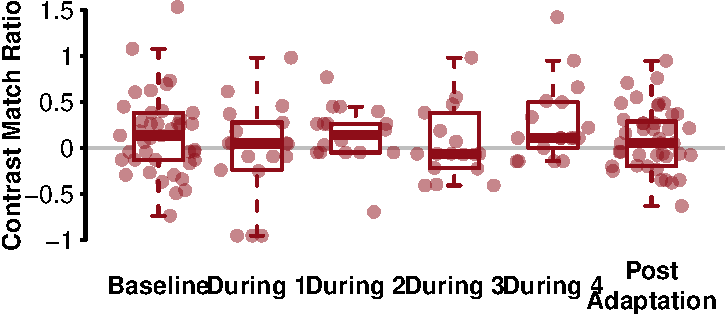
\includegraphics[keepaspectratio]{OrientationAdaptationPaper_files/figure-pdf/draw data boxplots-3.pdf}}

\pandocbounded{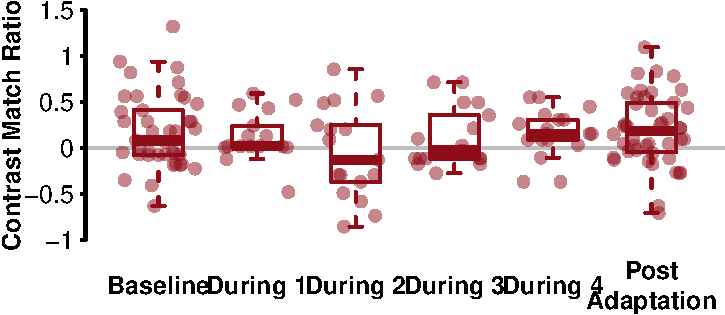
\includegraphics[keepaspectratio]{OrientationAdaptationPaper_files/figure-pdf/draw data boxplots-4.pdf}}

\pandocbounded{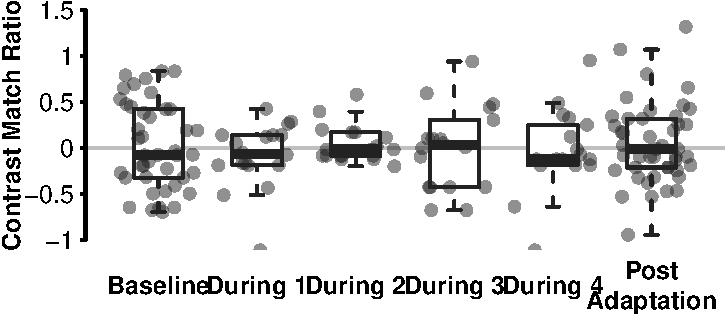
\includegraphics[keepaspectratio]{OrientationAdaptationPaper_files/figure-pdf/draw data boxplots-5.pdf}}

\pandocbounded{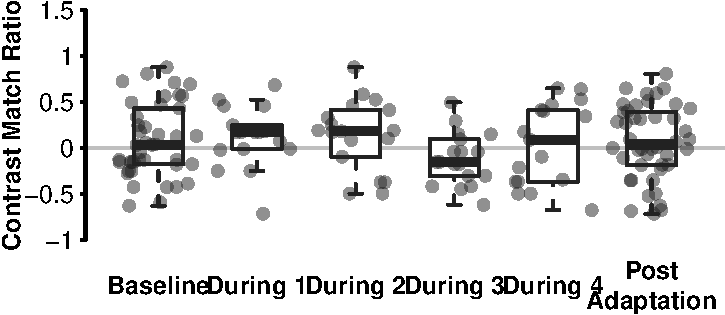
\includegraphics[keepaspectratio]{OrientationAdaptationPaper_files/figure-pdf/draw data boxplots-6.pdf}}

\pandocbounded{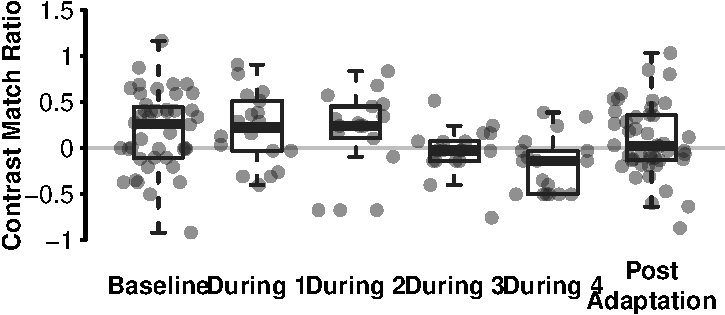
\includegraphics[keepaspectratio]{OrientationAdaptationPaper_files/figure-pdf/draw data boxplots-7.pdf}}

\pandocbounded{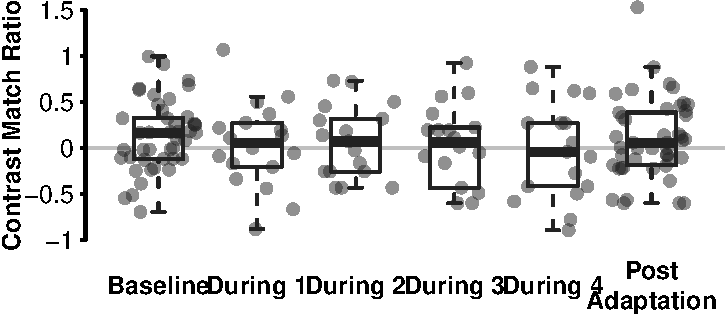
\includegraphics[keepaspectratio]{OrientationAdaptationPaper_files/figure-pdf/draw data boxplots-8.pdf}}

\pandocbounded{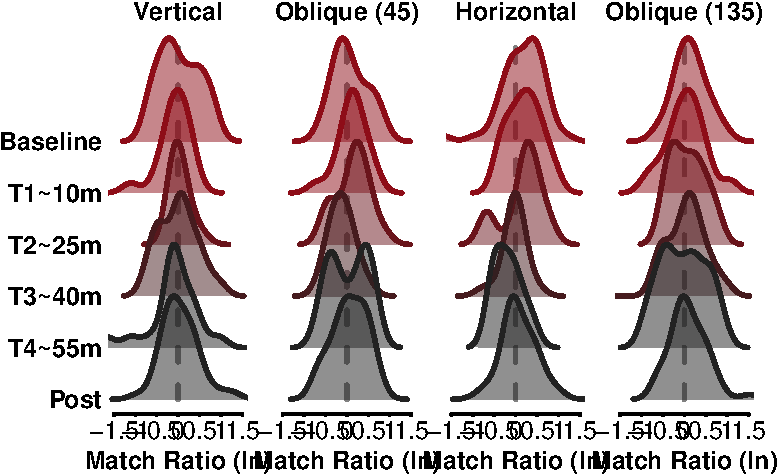
\includegraphics[keepaspectratio]{OrientationAdaptationPaper_files/figure-pdf/draw data distributions-1.pdf}}

\section{Modelling}\label{modelling}

\section{Discussion}\label{discussion}

\section{References}\label{references}




\end{document}
